\section{System Models}

After eliciting and specifying requirements, this section presents abstractions such as analysis models representing how the system satisfies these requirements.
The models do not depict the exact implementation.
Instead, they show a simplified conceptual representation of FLOps' architecture and workflows.
This includes involved components and their relationships.
The goal is to improve comprehension of the system instead of showing overwhelmingly verbose intricate details that might change in future updates.

System models aim to build what is called an analysis model.
The analysis model has three distinct parts.
Scenarios and use cases form the functional model.
Class and object models make the analysis object model.
State machines and sequence diagrams create the dynamic model of the system. \cite{book:bruegge}

\subsection{Use Case Model}

\begin{figure}[p]
    \begin{adjustwidth}{-0.1\paperwidth}{-0.1\paperwidth}
        \centering
        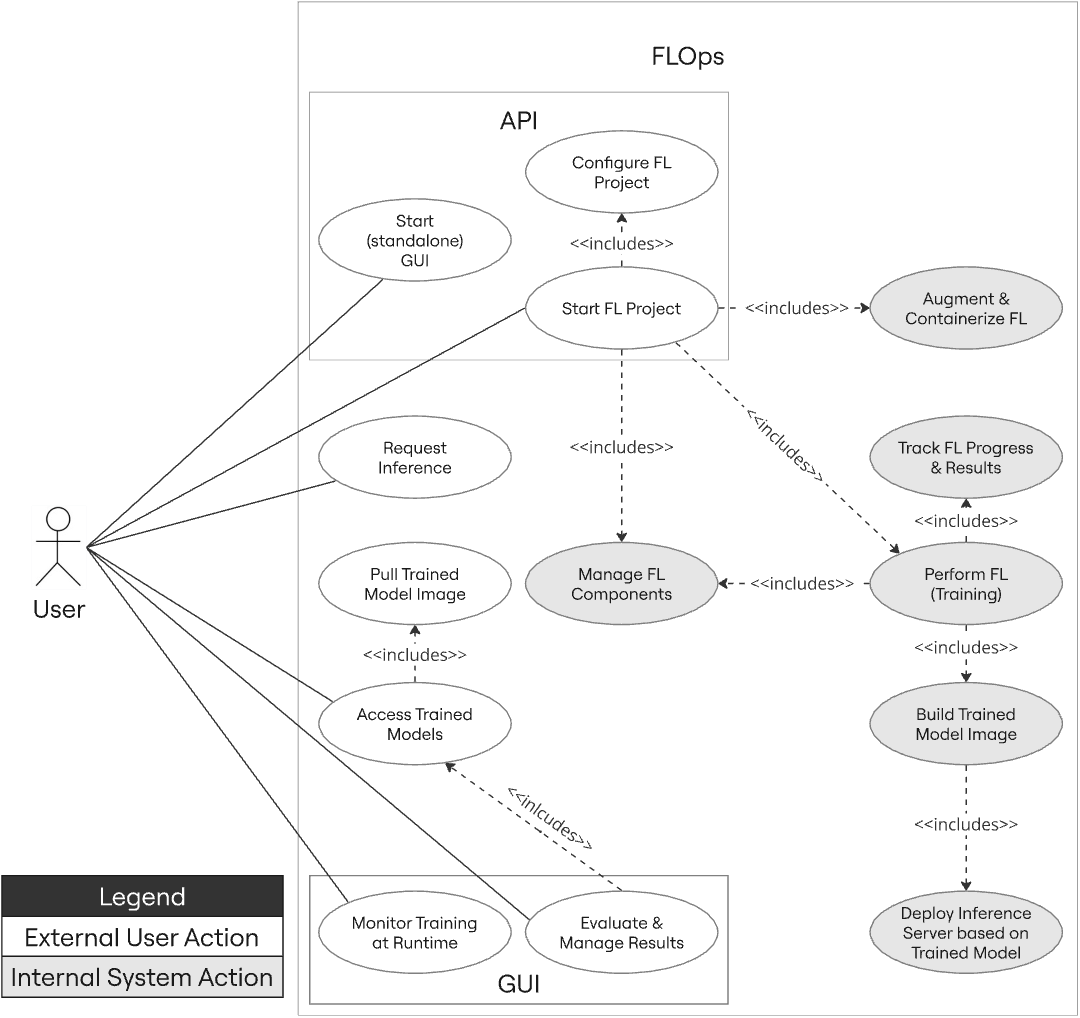
\includegraphics[width=0.9\paperwidth]{uml_use_case_diagram.png}
        \caption{FLOps UML Use Case Diagram}
        \label{fig:uml_use_case_diagram}
    \end{adjustwidth}
\end{figure}

Figure \ref{fig:uml_use_case_diagram} shows the Use Case diagram for FLOps.
The white use cases represent the functionalities the external users can directly trigger.
The grey use cases are internal system actions that are directly visible to users or lead to visible results.
They get triggered as a result of user actions.
For example, the user knows that FLOps is performing FL training by inspecting different provided outlets, such as the GUI.
FLOps tracks the training progress and results.
These logged artifacts become incrementally visible to the user who inspects the GUI.
Thus, the user knows that FLOps is currently performing FL training and logging.
Use cases inside the GUI boundary are directly accessible via the GUI. 
The same applies to the API boundary.
Other tasks are executed and accessible via FLOps combined with its orchestrator.
Use cases that involve developing or modifying FLOps itself are not explicitly portrayed.
The depicted User actor represents end users of varying FL expertise (\hyperref[FR-1.1]{FR-1.1}).
This actor includes FL developers and researchers.
The core use case is starting an FL project which also includes configuring that project (\hyperref[FR-2]{FR-2}).
This activity starts a chain of events, such as building an FL-enabled container image (\hyperref[FR-3]{FR-3}), creating and deploying the learners and aggregator(s), and performing the FL training (\hyperref[FR-1]{FR-1}).
During training, FLOps tracks the model and system metrics, which the user can monitor and evaluate in the GUI (\hyperref[FR-4]{FR-4}).
After training, the model can be containerized and deployed as an inference server (\hyperref[FR-5]{FR-5}, \hyperref[FR-6]{FR-6}).
The user can access this trained model (\hyperref[FR-5]{FR-5}) and request services from its inference server (\hyperref[FR-6]{FR-6}).


\subsection{FLOps Overview}\label{subsection:flops_overview}

\begin{figure}[H]
    \begin{adjustwidth}{-0.1\paperwidth}{-0.1\paperwidth}
        \centering
        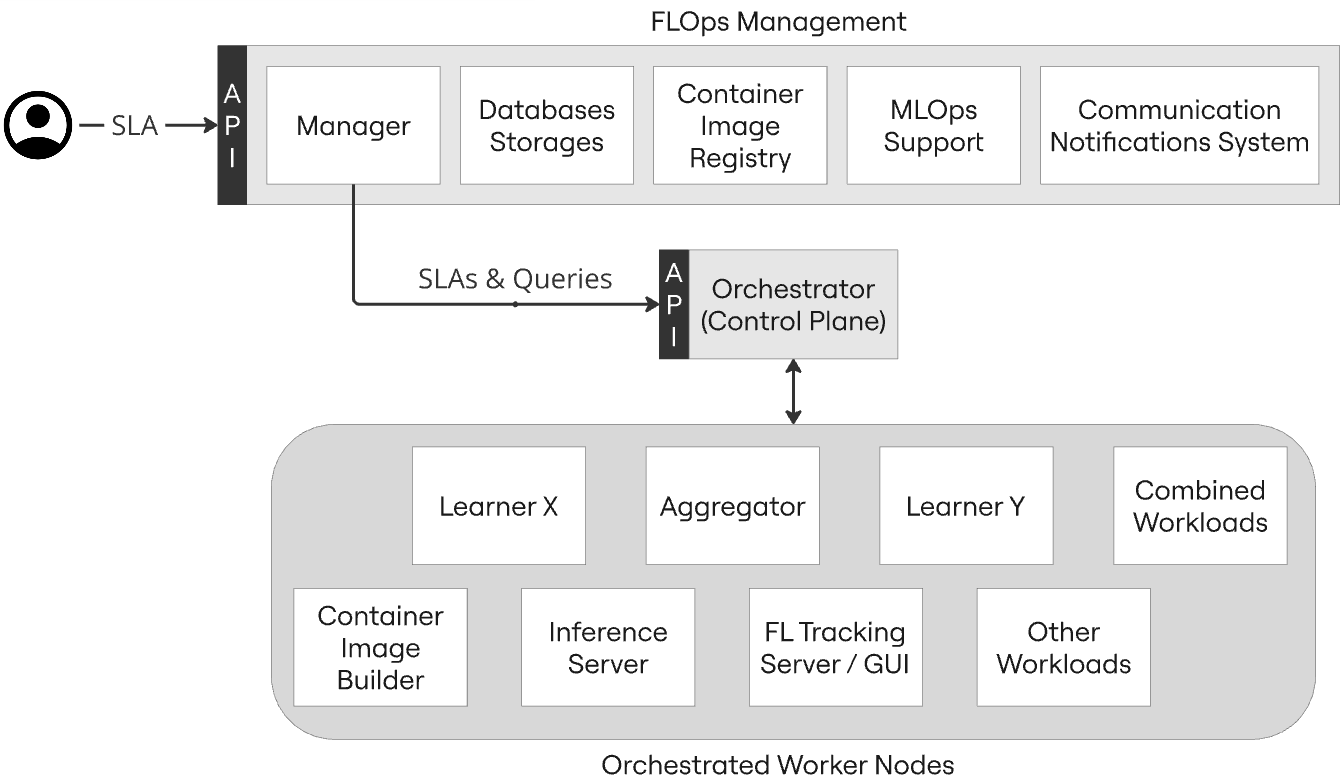
\includegraphics[width=0.8\paperwidth]{primer_flops.png}
        \caption{FLOps Structural Overview}
        \label{fig:flops_structure_overview}
    \end{adjustwidth}
\end{figure}

Figure \ref{fig:flops_structure_overview} provides a simplified overview of FLOps' structure.
Note that the management components and deployed services on orchestrated workers are interconnected.
These connections are not explicitly visualized to avoid clutter.
The services shown in the rounded rectangle depict an arbitrary number of worker nodes.
Multiple services can run on the same worker, or every worker might only have a single service deployed.
The FLOps system works via the interactions and relationships between the FLOps management, the orchestrator, and the worker nodes.
The FLOps management is a composition of components (containers).
Its goals and responsibilities are to manage FLOps processes and store FLOps artifacts.
The management components coordinate automatic processes and events.
They store container images and training results such as metrics and trained models.
These managerial components do not perform the FL training.
They delegate and distribute computation to orchestrated worker nodes.
The FLOps manager uses the orchestrator to create, (un)deploy, and remove different components.
The manager spreads computationally heavy image builds and FL training across the worker nodes.
The GUI and inference servers also run on worker nodes.

Figure \ref{fig:flops_simple_image_builder} shows a simplified overview of FLOps' image builder processes.
The container images get built on worker nodes.
Worker B stands for an arbitrary worker node capable of building images, i.e., the worker has enough resources and privileges.
The build process occurs inside a container that requires special considerations.
Remember that the user only provides ML code, not FL code.
FLOps' image builder clones the user ML code, augments it to support FL, handles specific dependency issues, and builds multi-platform container images.
This builder can build FL actors, i.e., the aggregator and learner images, as well as an inference server for the trained model.
These images get pushed to the FLOps image registry.
When the learners, aggregators, or inference servers are needed, their corresponding images are pulled from that registry onto an orchestrated worker node and executed.
Image builder services only exist when they are needed.
The FLOps manager removes them after building images for a concrete FLOps project.

\begin{figure}[h]
    \centering
    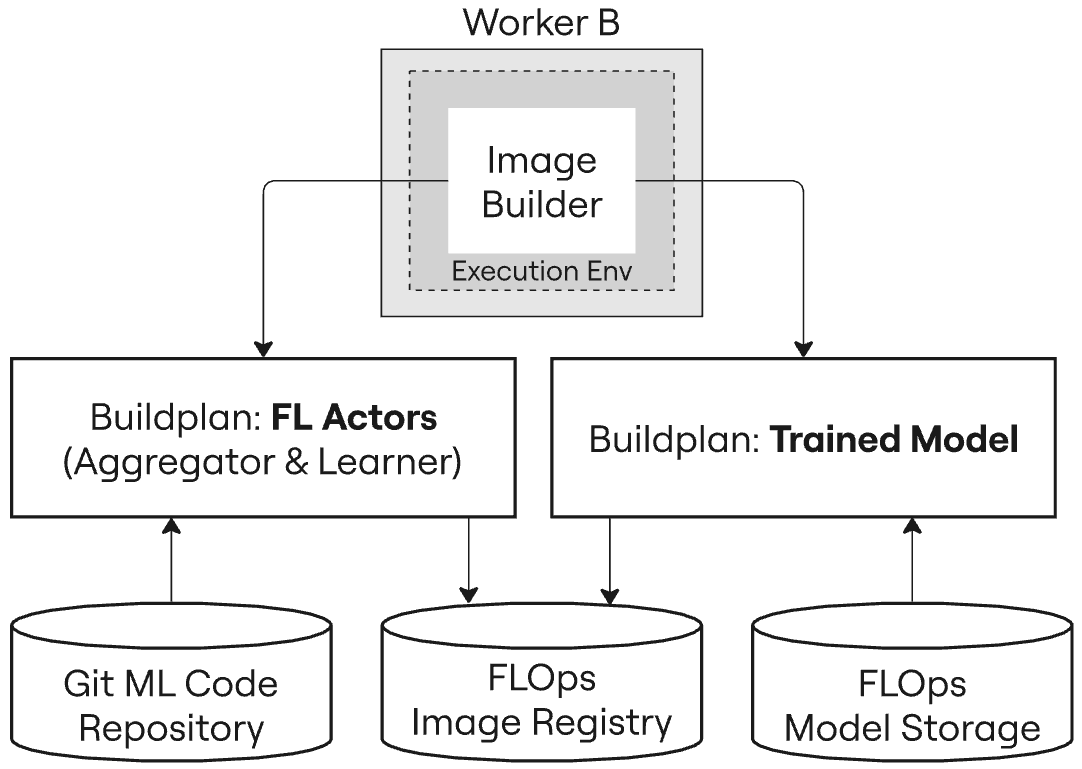
\includegraphics[width=0.8\textwidth]{simple_builder.png}
    \caption{Simplified FLOps Image Builder Processes}
    \label{fig:flops_simple_image_builder}
\end{figure}

\begin{figure}[H]
    \begin{adjustwidth}{-0.1\paperwidth}{-0.1\paperwidth}
        \centering
        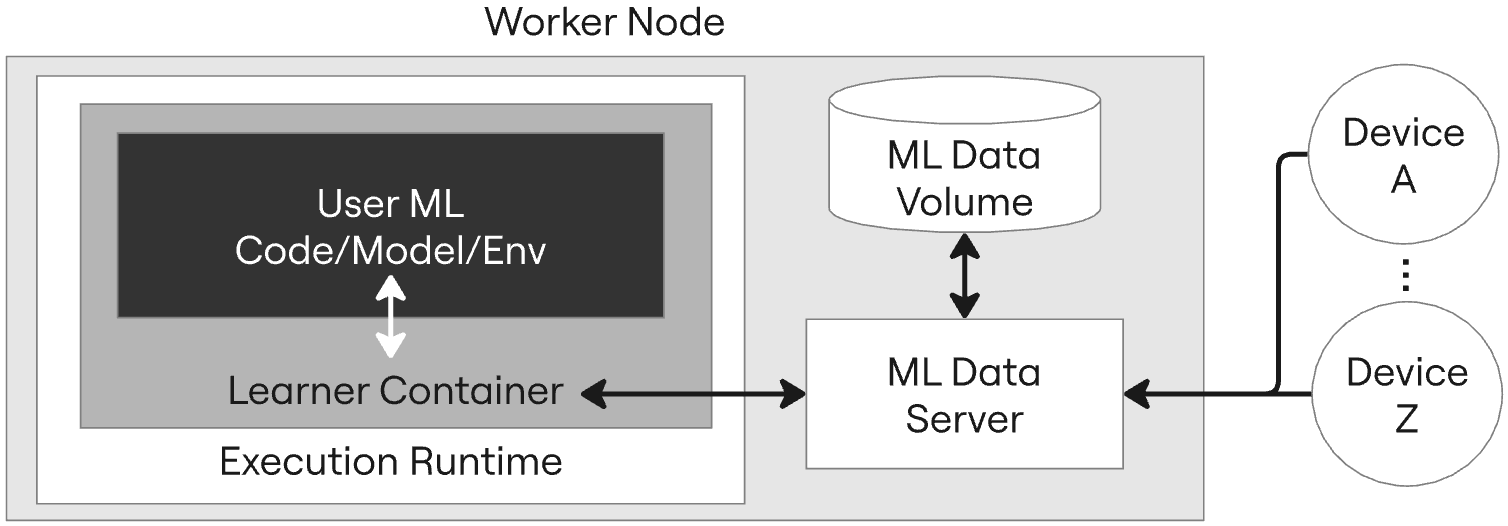
\includegraphics[width=0.70\paperwidth]{simple_data_management.png}
        \caption{Simplified FLOps Local Data Management}
        \label{fig:flops_simple_data_management}
    \end{adjustwidth}
\end{figure}

Figure \ref{fig:flops_simple_data_management} shows a simplified overview of how FLOps manages local training data.
FLOps targets practical, real FL applications.
Thus, it does not expect users to provide data as part of their ML repositories.
Instead, users need to coordinate with real data providers on the orchestrated worker nodes.
The figure shows a deployed learner container on a worker node.
The learner container itself has no data. 
FLOps cooperates with the orchestrator and deploys an ML data server before training on user-specified worker nodes.
This data server is reachable by nearby devices via an API.
Devices can send their data to this data server.
The data server will store this data on the local machine.
During FL training, the augmented learner container will fetch the local data via the data server.
The augmented learner FL code forwards this local data to the user ML code for preprocessing and training.
FLOps aims to support resource-restricted edge and IoT devices.
They are usually not capable of handling demanding ML training.
Letting them send their data to nearby edge/fog gateway devices capable of such tasks is possible.
This idea is similar to the approach in \cite{paper:global_fl_platform_for_iot}.




\subsection{Analysis Object Models}

This subsection depicts FLOps' main components and their relationships in more detail.
The following models are derived from and created to resolve the elicited requirements.
They focus on the user perspective.
It is common to use generalized and abstract UML class diagrams to depict the system's main components, properties, and functions \cite{book:bruegge}.

\begin{figure}[h]
    \centering
    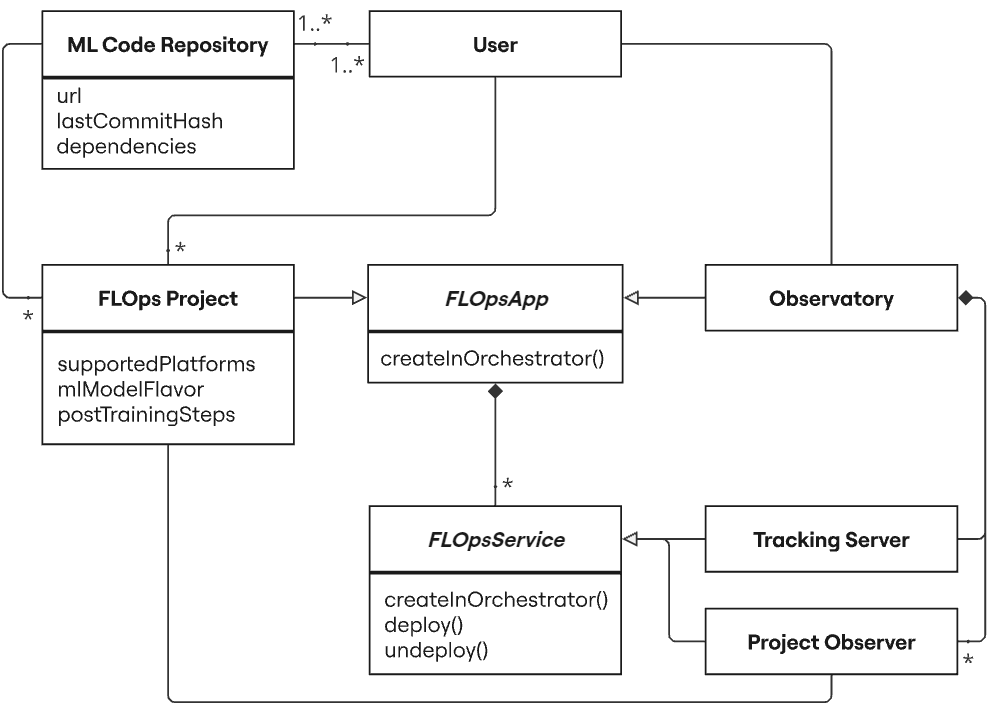
\includegraphics[width=1.0\textwidth]{uml_analysis_object_model_core.png}
    \caption{FLOps Core UML Analysis Object Model}
    \label{fig:uml_core_analysis_object_model}
\end{figure}

Figure \ref{fig:uml_core_analysis_object_model} shows the core FLOps UML analysis object model.
The main workflow is represented and grouped via a FLOps project.
Such a project links all necessary FL and ML/DevOps components to power one FL user request.
A project contains information about the user who requested it, the target platforms that should be supported (e.g., ARM/AMD), and what steps FLOps should perform after training.
If no steps are specified, the FLOps project counts as completed after training.
Available post-training steps include building a containerized image for the trained model and deploying an inference server to serve the trained model.
The ML model flavor indicator tells FLOps what ML framework to expect and work with.
Examples include Keras, Sklearn, or Pytorch.
Each project is associated with exactly one ML code repository.
This repository can be owned by the user or be a public one.
Thus, multiple users can reuse the same repository, and each user can create multiple FLOps projects per repository.
These properties are based on the SLA from the user request.

FLOps uses the concepts of applications and services to manage dependent components and concepts.
Each app can have multiple services.
Services are bound to parent apps and cannot exist on their own.
The orchestrator creates and realizes apps and services as usable components.
Applications themselves are collectors of information and metadata.
They do not run or contain any executable code, images, or similar.
Services are the computational components that can be deployed and un-deployed.
This split is based on Oakestra's applications and services.
The two main FLOps app types are project-based apps and customer-facing ones.

The observatory app is a customer-facing app.
There is exactly one observatory app for each user, whereas users can have multiple projects.
The observatory hosts the tracking server and project observer services.
The tracking server service tracks the projects and individual FL experiments.
It hosts the GUI. 
(It utilizes the MLFlow tracking server mentioned in \ref{subsection:mlflow}.)
When users request/start a new project, the observatory is created with all its components if it does not already exist.
Users can request access to the GUI/tracking server independently from a project.
A project observer service gathers and displays information or updates regarding the project status for the user.
The project observer informs the user of any issues during the project's live time, such as dependency issues during the containerized image builds.
There is one project observer per project to improve readability and comprehension.

\begin{figure}[t]
    \centering
    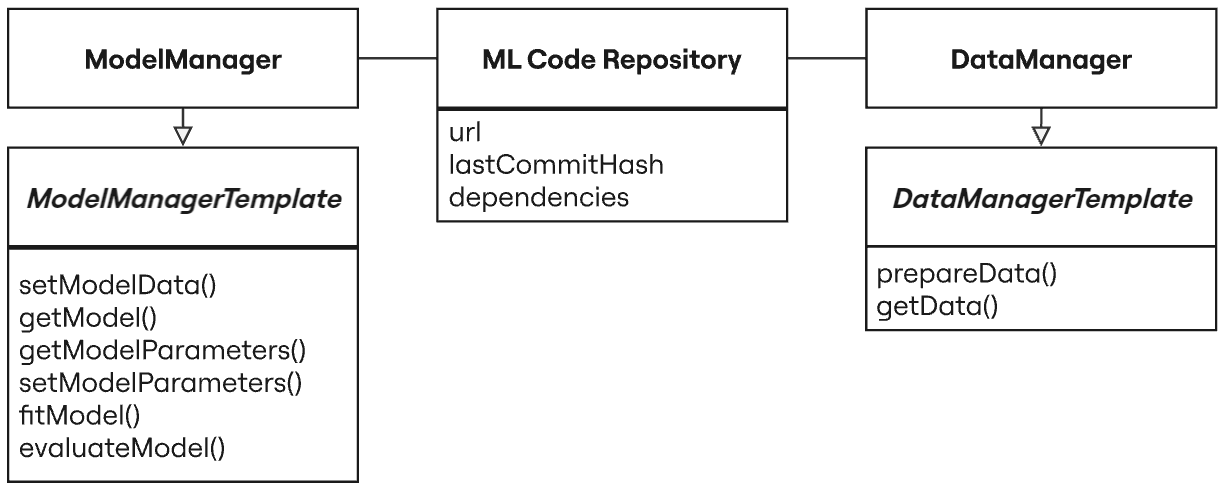
\includegraphics[width=1.0\textwidth]{uml_analysis_object_model_repo.png}
    \caption{FLOps ML Code Repository UML Analysis Object Model}
    \label{fig:uml_repo_analysis_object_model}
\end{figure}

Figure \ref{fig:uml_repo_analysis_object_model} shows additional details of the ML code repositories from the core model.
Users can provide a link to ML code repositories for FLOps to augment and train.
The repository must fulfill the following structural requirements for this to be possible and straightforward.
The repository needs a dedicated file that lists all necessary dependencies to train its model.
Theoretically, it should be possible to extract these requirements dynamically by inspecting the code.
However, this is a complex and error-prone endeavor.
To avoid these issues, users should provide the dependencies they used for training.
\vspace{5mm}
\newline
\textbf{Recommendation}: We recommend running the training locally on some exemplary or mock data and recording the dependencies via MLflow's auto-logging functionality.
This is an easy and viable approach to getting a suitable dependency file.
Note that this does not guarantee compatibility because MLflow's dependency logging can be erroneous.
Before providing the dependency file to FLOps, we recommend ensuring the dependencies are sufficient and compatible.
\vspace{5mm}
\newline
For FLOps to augment and utilize the ML code properly, FLOps requires the repository to implement a model manager and data manager.
The model manager is the interface that accesses the model and its data and parameters.
It further trains and evaluates the model.
It calls its linked data manager to prepare the data and retrieve it once it is ready.
The data itself should not be part of the repository.
The prepare data method will call a FLOps method that will be added during FL augmentation.
The user has to define in \texttt{prepareData} how to pre-process the retrieved data for individual training.
Both managers have an abstract parent class that users can import during implementation for guidelines.
These templates are available as part of the FLOps Utils pip package \cite{flops_utils_pip}.

\begin{figure}[t]
    \centering
    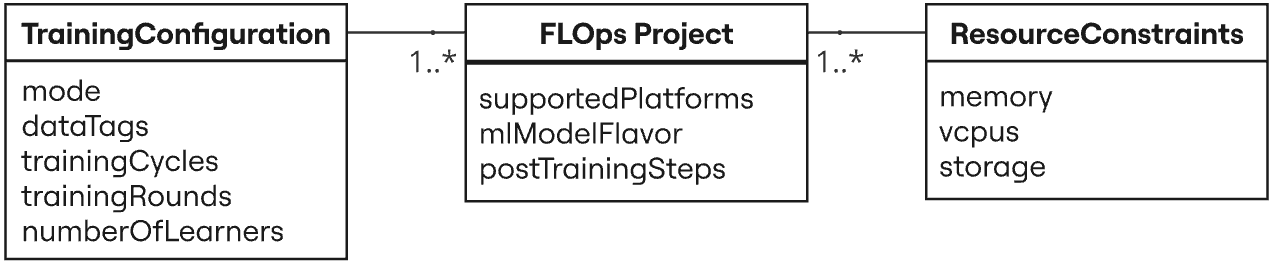
\includegraphics[width=1.0\textwidth]{uml_analysis_object_model_project.png}
    \caption{FLOps Project UML Analysis Object Model}
    \label{fig:uml_project_analysis_object_model}
\end{figure}

Figure \ref{fig:uml_project_analysis_object_model} shows further details about the contents of an FLOps project.
Users can customize their projects via the SLA (\ref{subsection:SLAs}) that is part of their API requests (\ref{subsection:api}).
One possible customization is to specify resource constraints such as memory or storage.
Users can customize the FL training by changing the project's training configuration.
The same ML repository can be trained differently depending on these configurations.
This configuration includes a mode that tells FLOps to perform different types of FL if applicable.
Currently, FLOps supports classic and (clustered) HFL.
The project will only use training data that matches the provided data tags.
The training rounds configure the number of training and evaluation rounds that each learner performs.
Only HFL uses training cycles.
The training rounds mean the number of training rounds performed on each learner per cycle.
A training cycle is the number of training rounds between the root and cluster aggregators, which resemble aggregators and learners in classic FL.
For example, if the user requests three cycles and five rounds, the learners will train five rounds per cycle for three cycles.
Each learner will train for 15 rounds during the entire project runtime.
The depicted attributes are only a subset of currently available and possible configurations.

\begin{figure}[t]
    \begin{adjustwidth}{-0.1\paperwidth}{-0.1\paperwidth}
        \centering
        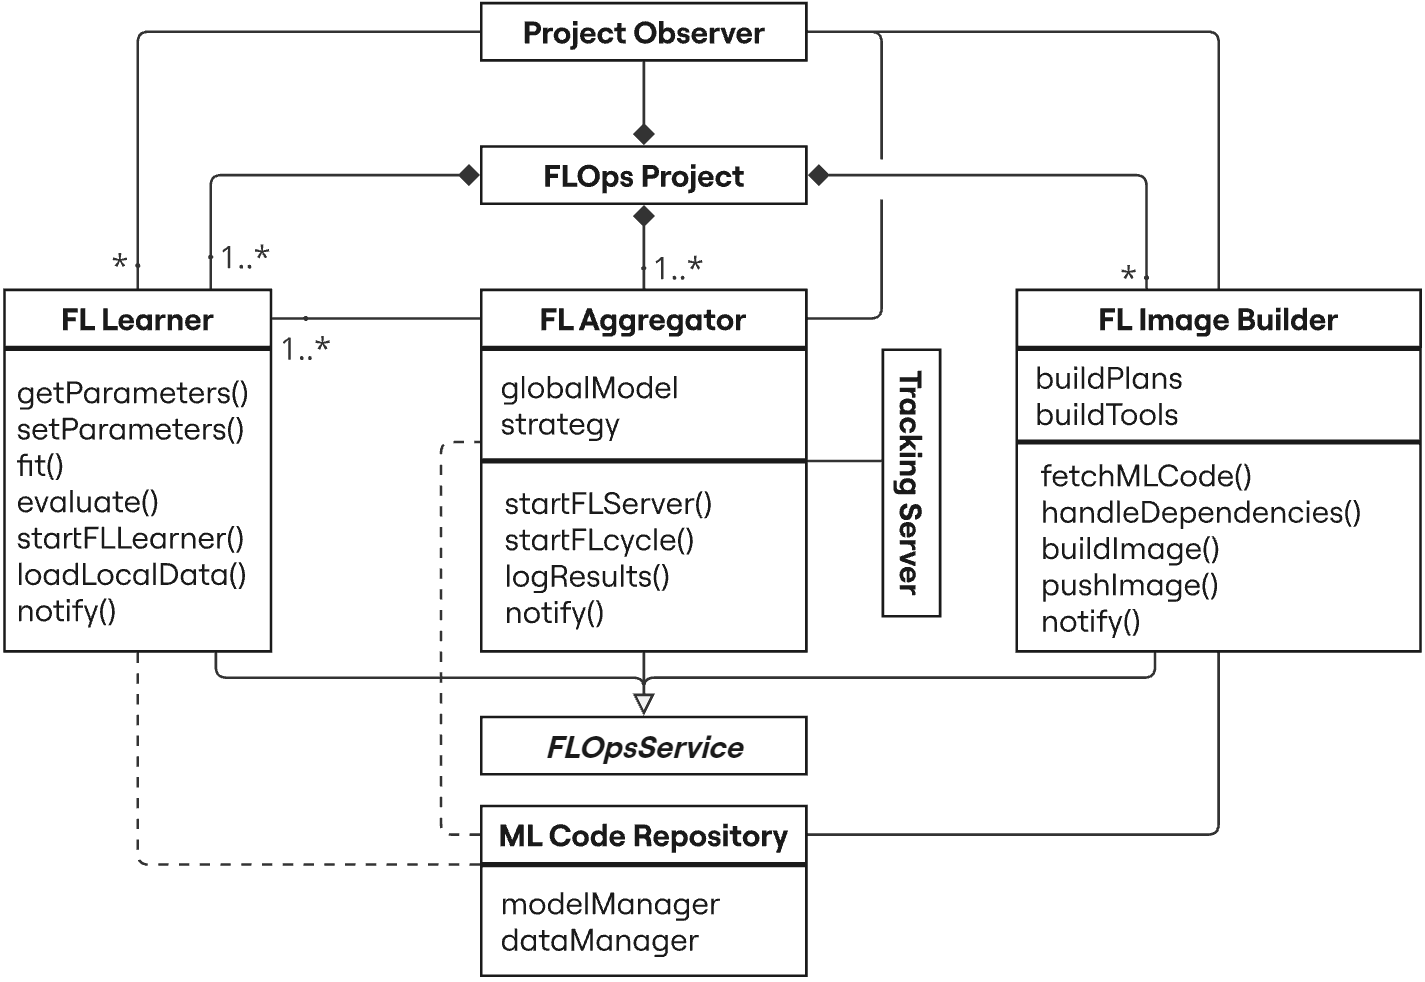
\includegraphics[width=0.80\paperwidth]{uml_analysis_object_model_project_services.png}
        \caption{FLOps Project Services UML Analysis Object Model}
        \label{fig:uml_project_services_analysis_object_model}
    \end{adjustwidth}
\end{figure}

The core figure \ref{fig:uml_core_analysis_object_model} only alluded that a project consists of several services and depicted only the project observer.
Figure \ref{fig:uml_project_services_analysis_object_model} expands upon this and shows important project services and their relationships.
There are three main project services.
The FL image builder is a service that builds containerized images.
It can build the FL augmented images for the learner, aggregator, and inference server of the trained model.
Different build plans enable this distinction.
The builder clones the ML repository, handles and checks the provided dependencies, builds the images, and pushes them to an image registry.
During and after the builder operation, the service notifies other components, including the project observer, about its progress, current state, and potential errors.

The FL aggregator manages the FL training loop and holds the global model and strategy for training.
It starts its internal FL server so learners can register for training.
The aggregator starts and terminates learning rounds and cycles.
It logs results like metrics or the final trained model via the tracking server.
Similarly to the builder, it notifies other components during runtime about its progress and errors.
The aggregator and learners utilize the code provided in the user's ML code repositories.
They have direct access to the model and data managers.
The image builder injects both of them.

The FL learners are project services that perform the FL training on local data.
They fetch locally stored data, connect to the aggregator, and perform FL activities such as training.
The learner uses the code found in the model and data managers and wraps itself around their implemented interface methods.
As a result, users do not need to implement the FL (boilerplate) code themselves.
Therefore, a learner's \texttt{getParameters} method uses the \texttt{getParameters} method described in the user's ML repository with additional logic around it.
Learners also notify other components about their progress or failures.

\begin{figure}[t]
    \centering
    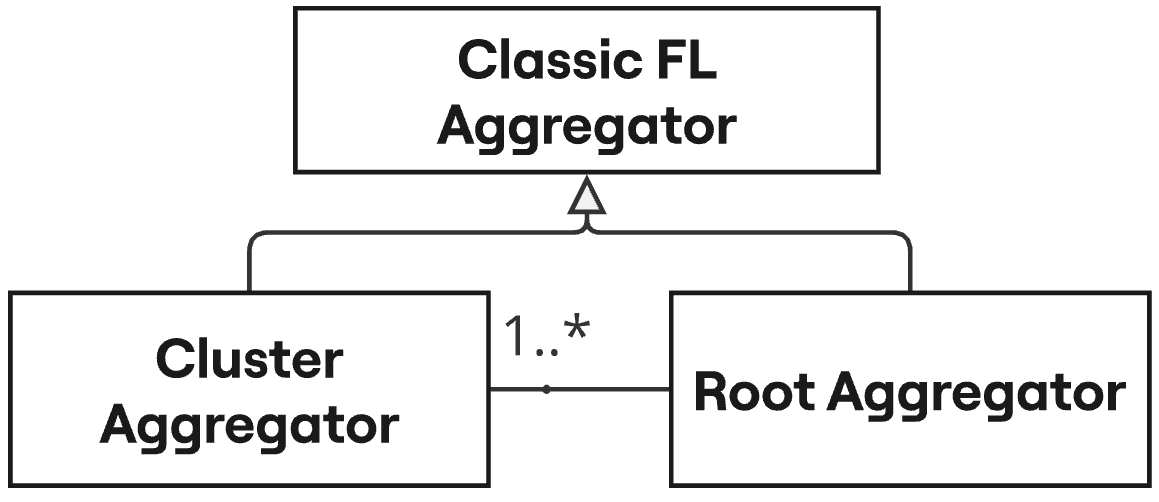
\includegraphics[width=0.55\textwidth]{uml_analysis_object_model_aggregators.png}
    \caption{FLOps Aggregator Types UML Analysis Object Model}
    \label{fig:uml_project_aggregators_analysis_object_model}
\end{figure}

Figure \ref{fig:uml_project_aggregators_analysis_object_model} shows the simplified relation between different FLOps aggregator types.
Because FLOps supports classic and hierarchical FL, it must support different aggregator types.
For conventional FL, FLOps uses the classic aggregators.
For HFL, FLOps creates a single root aggregator and one cluster aggregator per cluster, which are available in the orchestrator.
The root orchestrator sees cluster orchestrators as plain learners.
A cluster aggregator is a hybrid between an aggregator and a learner.

\subsection{Dynamic Models}

Dynamic models illustrate the dynamic behavior of the system and the interactions between its components.
Different dynamic model types include UML activity, state chart, communication, and sequence diagrams.
Because of the large number of components in FLOps, this section focuses on sequence diagrams to cover a large set of significant interactions.

This subsection depicts the necessary interactions for a typical FLOps project.
We use many abstractions and depict the absolute base case for an FLOps project to reduce complexities and improve readability.
The base case aims to showcase a project workflow from the ground up.
That means that no code, data, or images are present yet.
This base case terminates after successful training.
It has no post-training steps, such as building and deploying an inference server.
FLOps management consists of multiple components.
For simplicity's sake, these components are grouped into one. 
The same applies to multiple worker nodes and edge devices.
To improve readability and comprehension we split up the project into stages.



\subsubsection{0. Preparation}

\begin{figure}[t]
    \begin{adjustwidth}{-0.1\paperwidth}{-0.1\paperwidth}
        \centering
        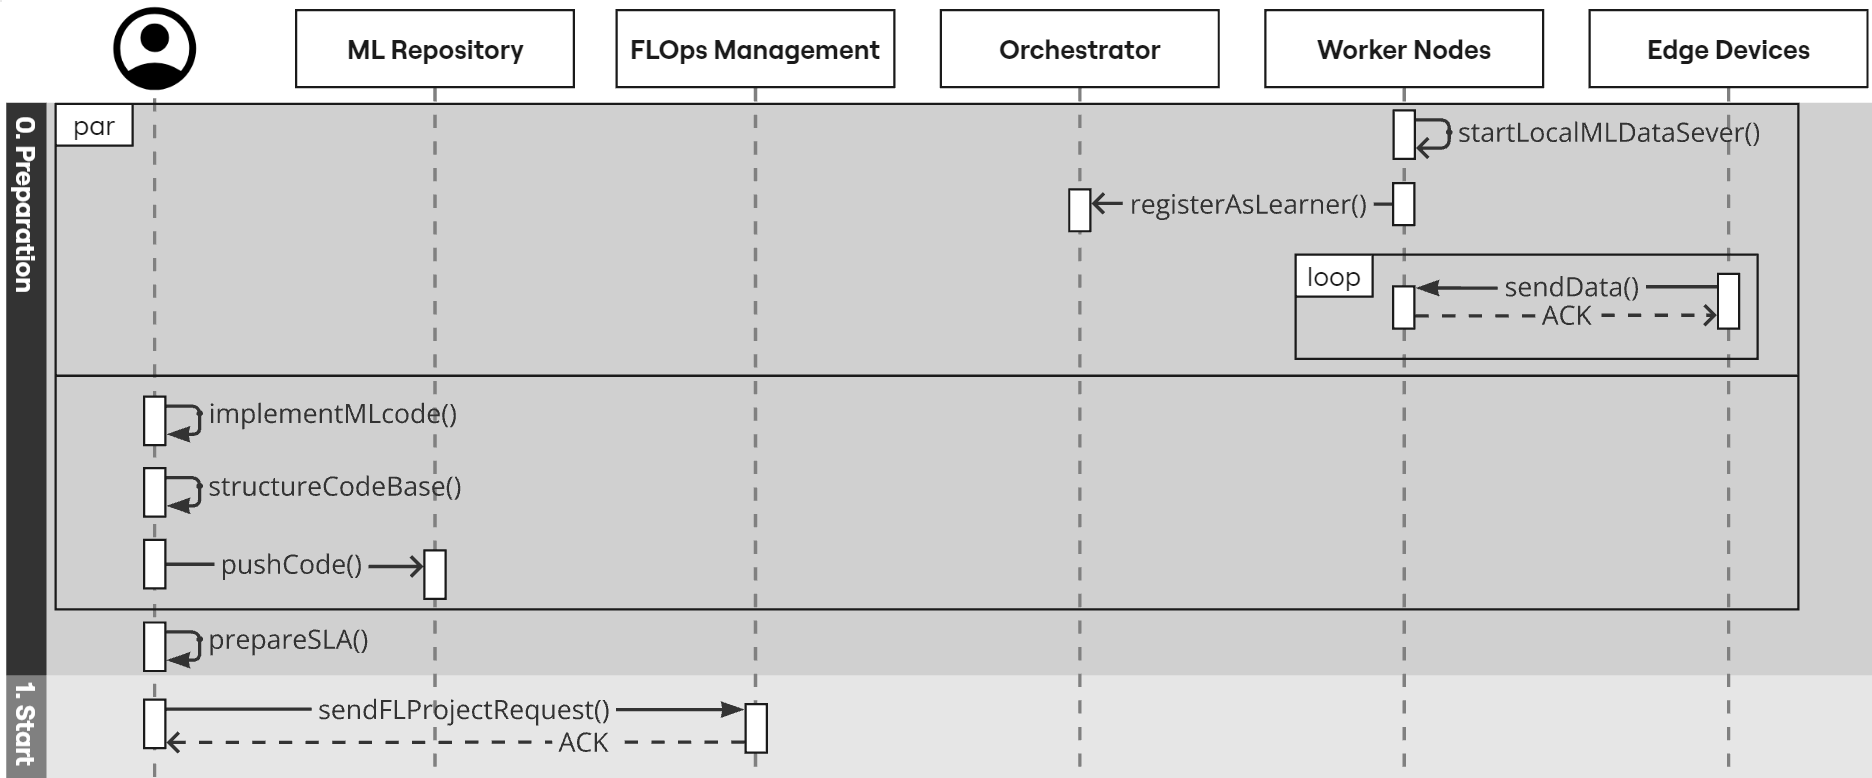
\includegraphics[width=0.9\paperwidth]{uml_sequence_init.png}
        \caption{FLOps Preparation - UML Sequence Diagram}
        \label{fig:uml_sequence_init}
    \end{adjustwidth}
\end{figure}

Figure \ref{fig:uml_sequence_init} is a UML sequence diagram depicting the initial steps before a FLOps project can start.
Two different sets of sequences can occur independently or in parallel with each other.
Before FLOps can run properly, FL worker nodes need to register with the orchestrator and stay available.
Only a subset of worker nodes are intended to be capable of performing ML training.
Worker nodes that should participate as learners must inform the orchestrator accordingly and start the provided ML data server locally.
This server accumulates training data locally for later training.
This process has to occur before training begins.
Otherwise, not enough or no data will be available for training.
Edge devices or other nearby data sources should send their data to these designated learner nodes.
The infrastructure provider has to ensure that these worker nodes are appropriately protected and trustworthy.
Once these steps are completed, FLOps should have access to available data-rich orchestrated worker nodes.

The second set of tasks that should occur before using FLOps is for users to prepare their ML code.
They should implement their ML code and structure it as required for FLOps.
This code must be available via an accessible git-based repository.
If the user is satisfied with his codebase, he can prepare his SLA.
(We discuss the SLA in detail in the implementation chapter.)
After both sequences have been completed, the user can send his SLA to the FLOps management API and request the start of a new FLOps project.

\subsubsection{1. Project Start}

Figure \ref{fig:uml_sequence_project_start} shows the main sequence of steps from starting a new FLOps project to deploying an image builder service.
The light blue activity bars mean that FLOps creates a new object inside the manager context, independent of the orchestrator and deployed components.
Management objects hold stateful information and are not run or used for computational workloads.
This split is necessary for the FLOps management to keep track of ongoing processes, retain memory, and handle unique custom requirements independent of and unavailable in the orchestrator.
Each colored or white rectangle on a lifeline inside the central UML sequence diagram corresponds to a specific functionality.
When this functionality terminates, the bar stops as well.
Usually, sequence diagrams show concrete instances of classes as actors.
We use abstract actors to optimize the page space and allow further abstractions and simplifications.
For example, the lifeline of an observatory app inside the orchestrator could be a separate actor.
However, this would lead to redundancy and verbosity between the orchestrator and observatory actors.
Instead, these modified graphs show the lifeline of FLOps components on the right side.
The color and dotted lines help to link those concepts together.
Light rose orchestrator actions symbolize a service being appended to an existing application.

The FLOps Management registered the new project request and extracted the SLA.
Firstly, the FLOps management creates a new observatory for the user inside the FLOps management context.
The management requests to create a corresponding app inside the orchestrator.
The same applies to the actual FLOps project.
When these two parent applications exist, the management will create the first service.
The management requests the creation of the project observer as a service inside the observatory application.
The management then requests to deploy an instance of this service on a worker node to the orchestrator.
Now, the user can access this project observer service at any time to observe the progress of his project.

The FLOps management checks if its image registry already contains images that match the requested ML repository.
For this, the management contacts the ML repository to check its latest state.
In this example, the registry is empty.
Therefore, new images are required.

\begin{figure}[t]
    \begin{adjustwidth}{-0.2\paperwidth}{-0.2\paperwidth}
        \centering
        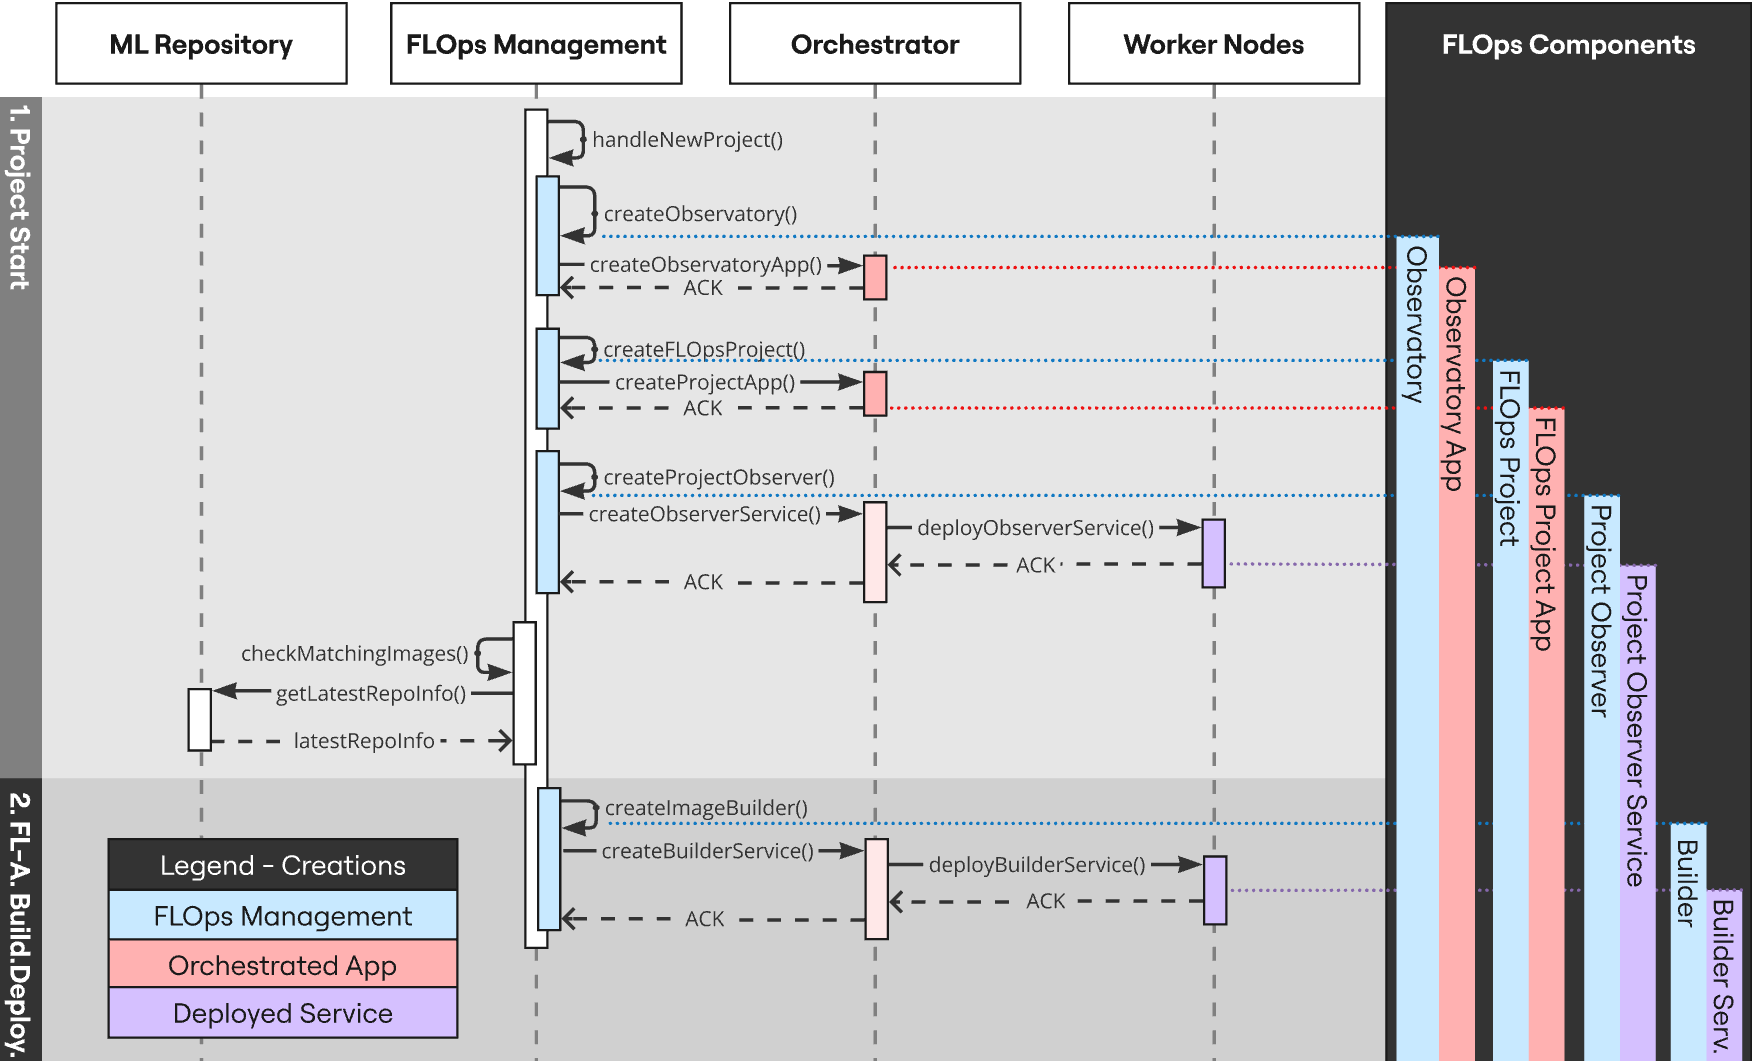
\includegraphics[width=0.95\paperwidth]{uml_sequence_diagram_project_start.png}
        \caption{FLOps Project Start - UML Sequence Diagram}
        \label{fig:uml_sequence_project_start}
    \end{adjustwidth}
\end{figure}

\subsubsection{2. FL-Actors Image-Builder Deployment}
The management creates a new image builder service and deploys it similarly to the project observer.

\subsubsection{3. FL-Actors Image Build}

\begin{figure}[t]
    \begin{adjustwidth}{-0.2\paperwidth}{-0.2\paperwidth}
        \centering
        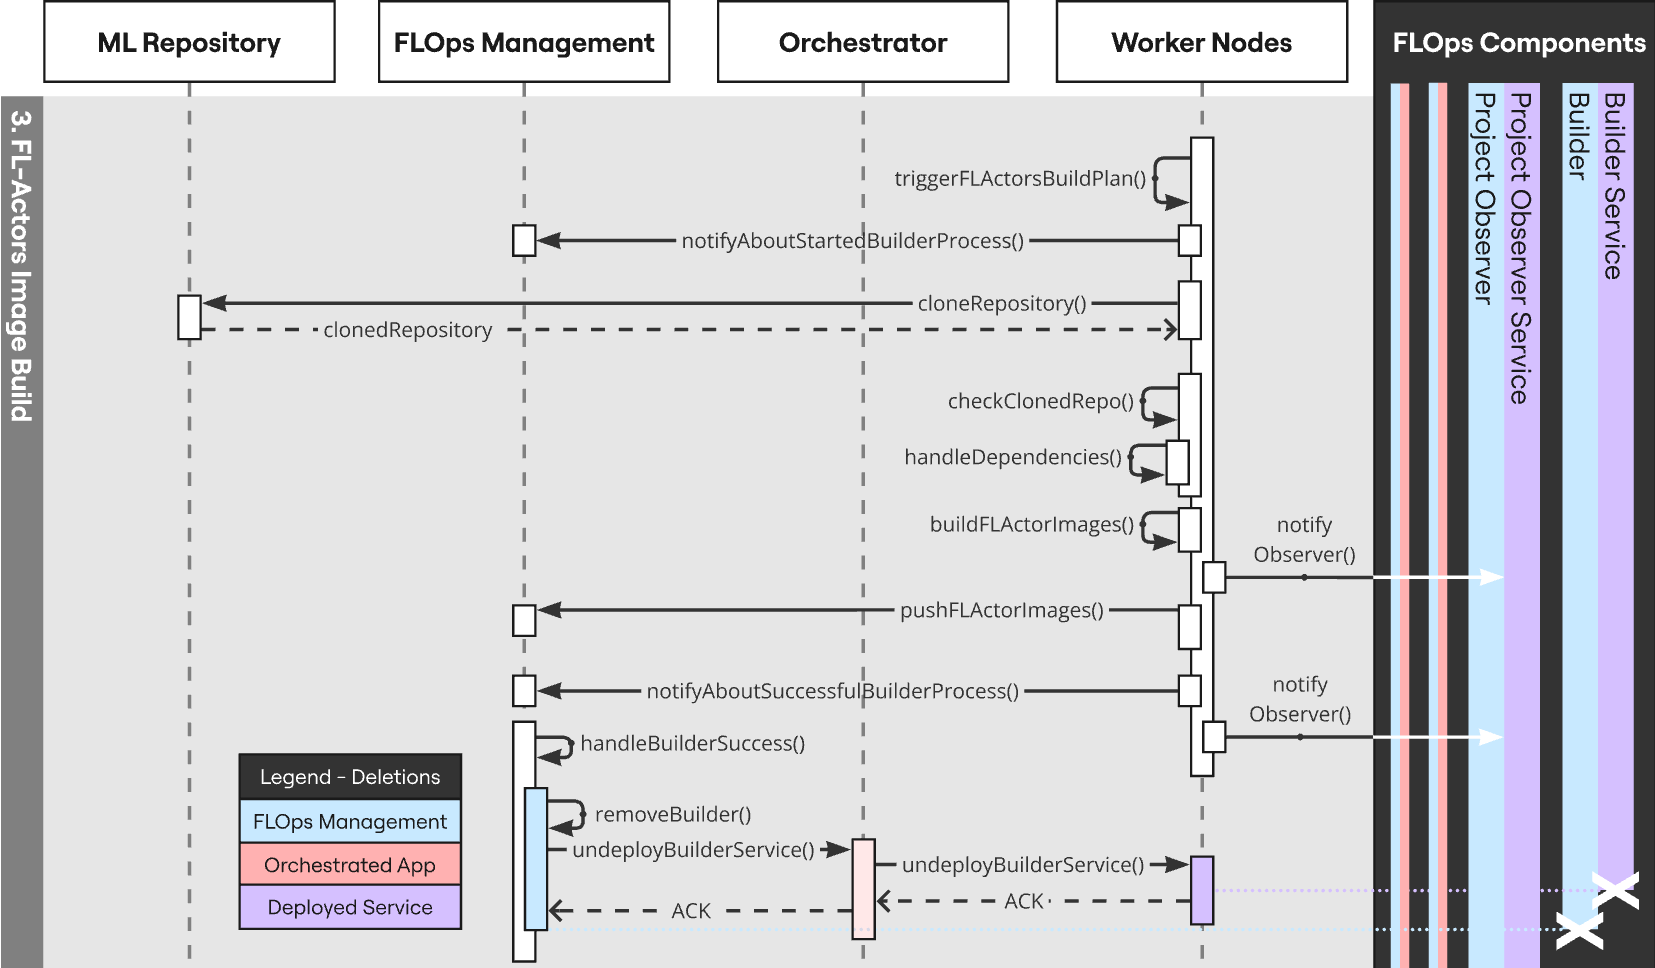
\includegraphics[width=0.95\paperwidth]{uml_sequence_actor_builder.png}
        \caption{FLOps Image Builder Processes - UML Sequence Diagram}
        \label{fig:uml_sequence_builder}
    \end{adjustwidth}
\end{figure}

Figure \ref{fig:uml_sequence_builder} shows the interactions necessary to augment user ML code into FL-enabled containerized images.
Once the builder service is deployed, it executes the build plan for actor images.
FL actors are the aggregator(s) and learners.
The builder service notifies the management about a successful start of this process.
It proceeds by cloning the ML repository and checks if it complies with FLOps requirements.
The builder also checks if the dependencies are sound.
When these build prerequisites are met, the builder continues to build the aggregator and learner images.
(Concrete details about this build process are available in the implementation chapter.)

Afterward, the builder notifies the project observer to inform the user about the successful build.
Note that the sequence model action lengths do not correspond to their actual duration.
Short rectangles visualize the build and push actions in the diagram, even though these two actions are by far the most time-consuming.

As the last build process step, the builder pushes these built images to the image registry hosted by the FLOps management.
After the successful push, the builder notifies the project observer and FLOps management of its successful completion.
The FLOps management catches this message and removes the builder from its own context and undeploys it from the orchestrator and worker.
Now that the FL actor images are ready, the training can begin.

\begin{figure}[p]
    \begin{adjustwidth}{-0.2\paperwidth}{-0.2\paperwidth}
        \centering
        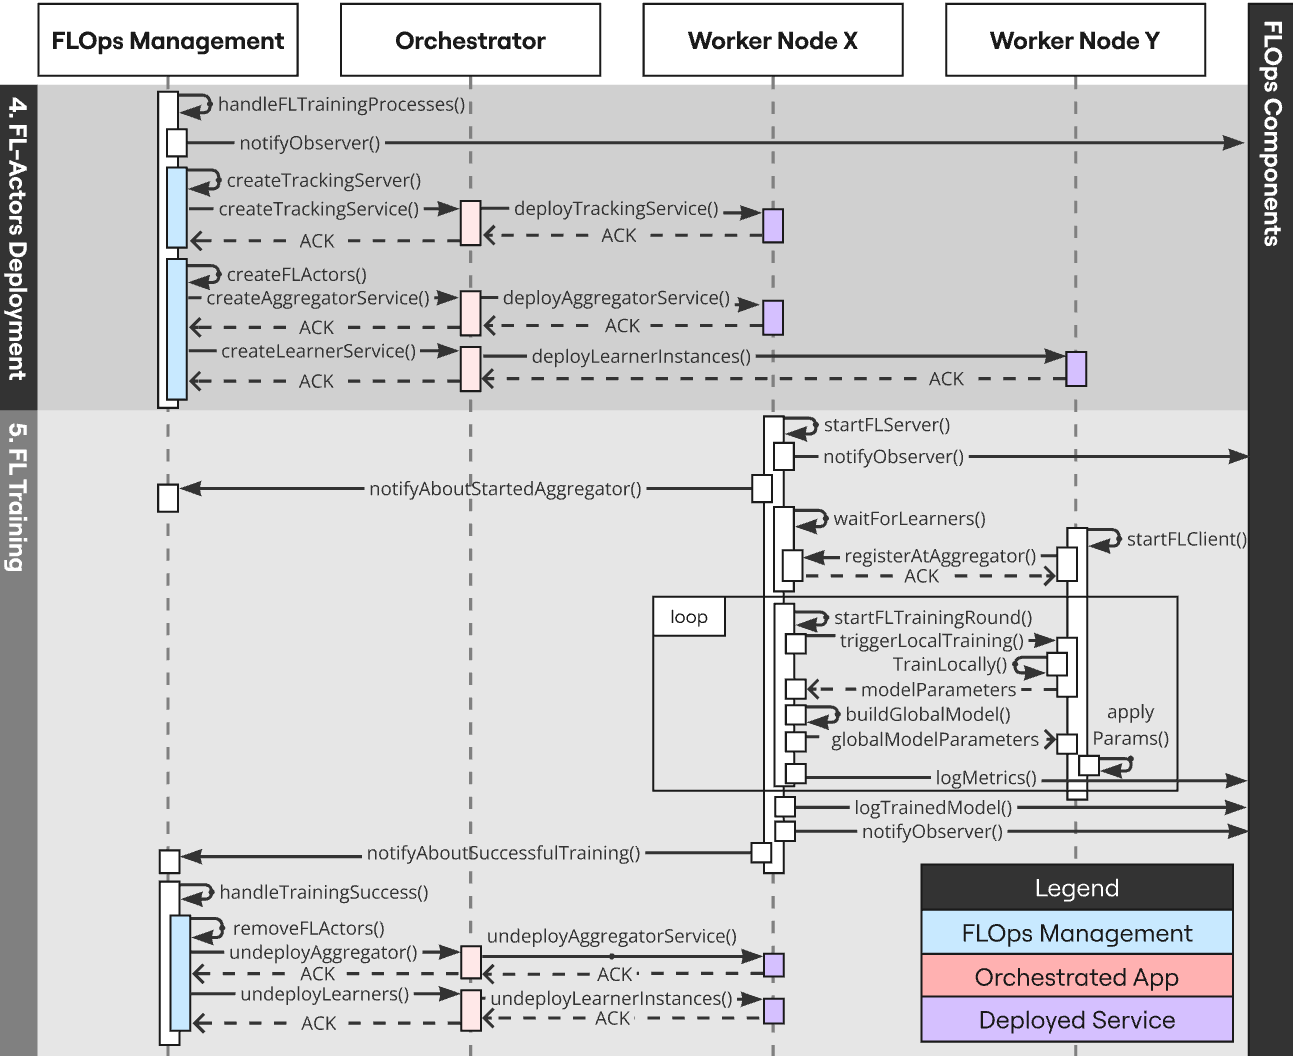
\includegraphics[width=0.95\paperwidth]{uml_sequence_training.png}
        \caption{FLOps FL Training Processes - UML Sequence Diagram}
        \label{fig:uml_sequence_training}
    \end{adjustwidth}
\end{figure}

Figure \ref{fig:uml_sequence_training} shows the necessary interactions that realize FL training under FLOps.
Note that the right side omits the previously depicted detailed FLOps component lifelines.
We collapse these details for this diagram because the depicted components and their lifetimes show similar behavior as the previous diagrams.
Arrows that point to the right mean that specific FLOps components are targeted.
They are not explicitly depicted to optimize readability and reduce verbosity.

\subsubsection{4. FL-Actors Deployment (Aggregator Deployment Stage)}
After building the required images, the FLOps management will start handling the FL training processes.
Firstly, it notifies the project observer that FL training will start shortly.
Secondly, it creates and deploys the tracking server that provides the GUI.
Users can access this GUI by following the link shown in the project observer or directly accessing the deployed tracking service, similarly to the project observer.
Note that there are several differences between the project observer and the GUI.
The project observer is a minimalistic way to inform the user about the current state and potential errors during the lifetime of an FLOps project.
The GUI is a standalone application that focuses on tracking the training results.

The FLOps management now creates and deploys the FL aggregator and learners.
It uses the previously built images for this.
Once the aggregator image is pulled and executed, it starts the FL server processes and notifies its watchers about its success.
The aggregator waits for learners to connect before starting the training.
In the meantime, the FL learner images were pulled and started.
Each learner starts its FL client activities, such as registering with its specified aggregator.

\subsubsection{5. FL Training}
Now that all FL actors are ready, the aggregator starts the first training round and triggers the learners.
The learners train their models with the local data from their worker node.
When completed, the learners will push their model parameters to the aggregator.
The aggregator fuses them into a new global model and returns the new global parameters to the learners.
The learners apply those to their local model to be ready to begin the next FL training round.
After each FL training round, the aggregator logs metrics, such as accuracy and loss, via the tracking server service.
The FLOps management stores the logged results.

After the last FL training round, the aggregator notifies its observers and logs the final trained model via the tracking service.
The aggregator only tracks the model a single time to avoid wasting bandwidth or storage.
Afterward, the aggregator and learner activities terminate.
Similarly to the builder's un-deployment process, the FLOps management registers the successful message and removes the FL actors.
With this, the core FLOps project is concluded.

\subsubsection{Further Stages}
Similarly, FLOps realizes more complex configurations, modes, or post-training steps.
For the post-training steps, the builder gets deployed again.
This time, it runs the trained model build plan and pulls the model from the FLOps management.
It pushes the built image back to the management image registry.
The inference service gets deployed similarly to the FL actors using the built trained model image.



